\subsection{Improvements to the Slimplectic Integrator and their Physical Applications}
\label{sec:results-si}

\begin{figure}[t]
  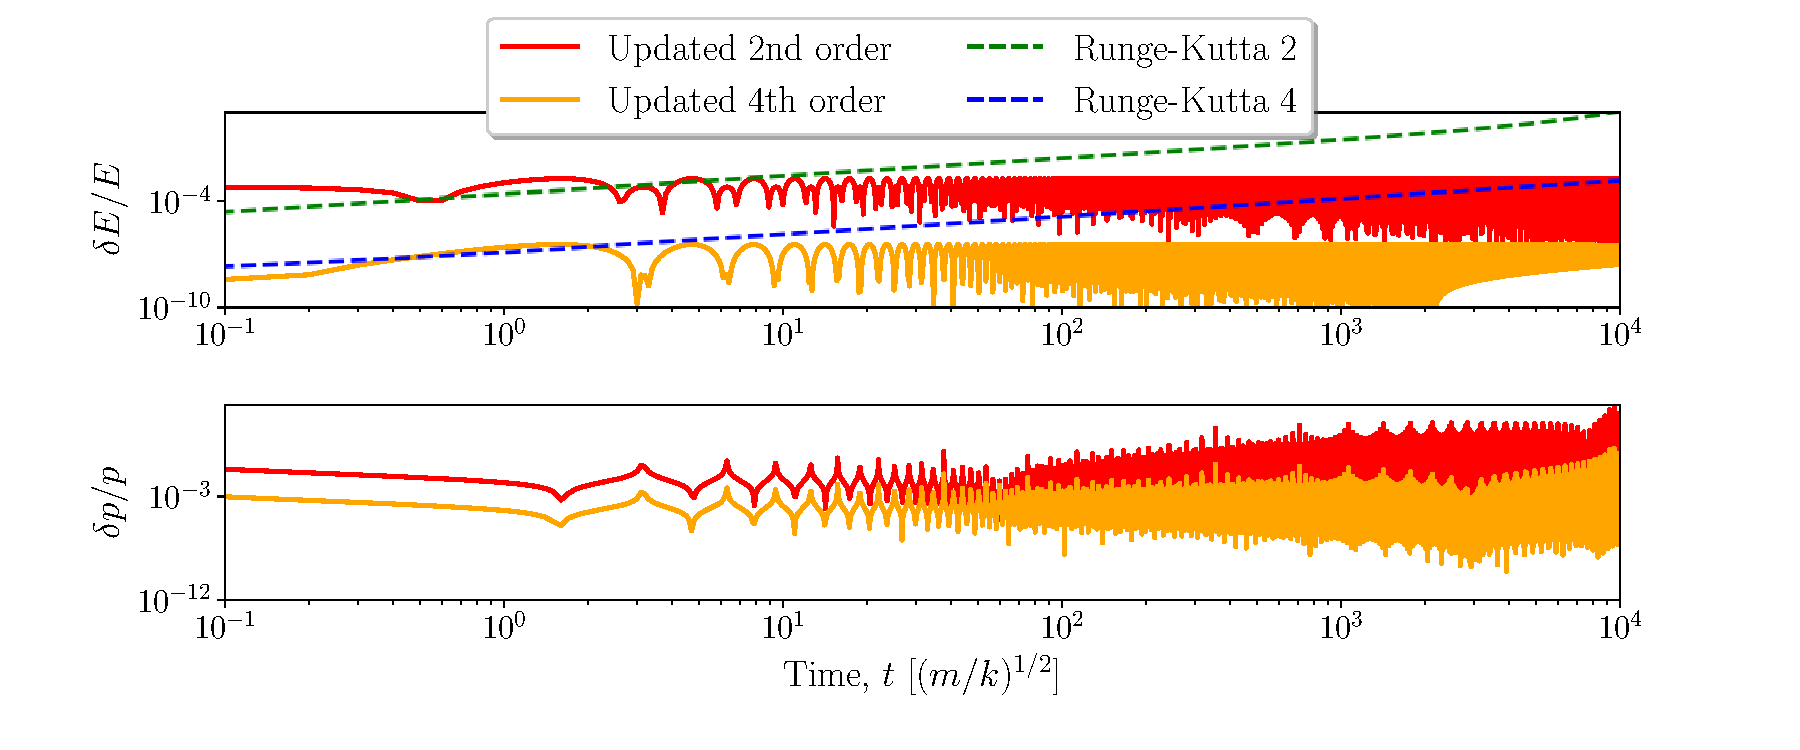
\includegraphics[width=\columnwidth]{figures/dho_energy_momenta_fractional_err.pdf}
  \caption{A comparison of the error in the energy, top, and momenta, bottom, as a fraction of the known analytic solution of the system, of the \updimpl{} simulating a damped harmonic oscillator. One can observe that the fractional energy error is bounded and displays the oscillating behaviour that we expect from previous work, whereas the momenta error does not display such behaviour. This plot is based on its equivalent in the original paper \cite[Figure 2, bottom]{tsangSLIMPLECTICINTEGRATORSVARIATIONAL2015}.}
\label{fig:dho_energy_bounds}
\end{figure}

As discussed we first verify that the \updimpl{} retains the required fractional error bounds of the formal method. This can be seen in \fref{fig:dho_energy_bounds} where the fractional error of the \updimpl{} with respect to that of the true analytic solution is compared directly against that of Runge-Kutta order 2 and 4. We clearly observe that the fractional energy error remains bounded across the timeframe of iteration.
This successfully replicated the behaviour of the original implementation to an absolute root mean squared residual over the simulation duration of $\Delta = 1.42 \times 10^{-13}$ and $\Delta = 4.50 \times 10^{-12}$ for $r = 2$ and $r = 4$ respectively.
This is not the case for the fractional momenta error however as fixed-time-step variational methods such as those implemented cannot be both slimplectic-momentum and momentum-energy preserving \cite{zhongLiePoissonHamiltonJacobiTheory1988}.

\begin{figure}[t]
  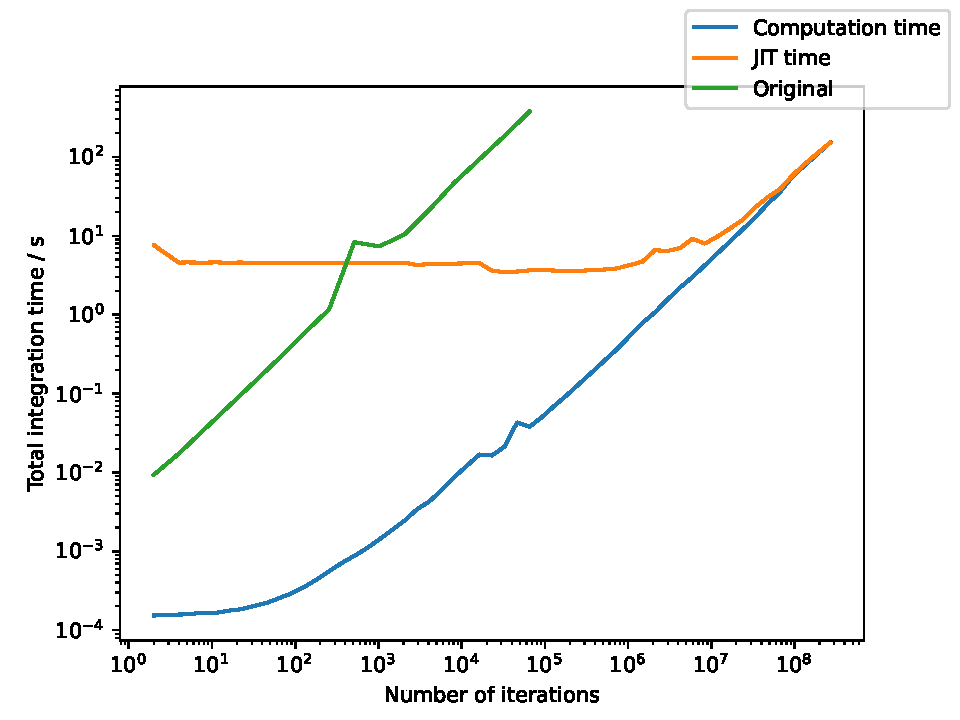
\includegraphics[width=\columnwidth]{figures/dho_n_runtime.pdf}
  \caption{A comparison of running a damped harmonic oscillator system for various numbers of iterations, with $r = 2, \Delta t = 0.1$. The \updimpl{} runtime is split into two components where \ensquote{JIT time} represents the one-time fixed cost of compiling the function (see \sref{sec:intro-autodiff}) and \enquote{Computation time} represents the actual time spent on computation.
  Each value is the mean of 4 runs, with the \orgimpl{} being cut off early due after $> 20$ minutes runtime for the next sample.}
  \label{fig:dho-n-runtime}
\end{figure}

\begin{figure}[t]
  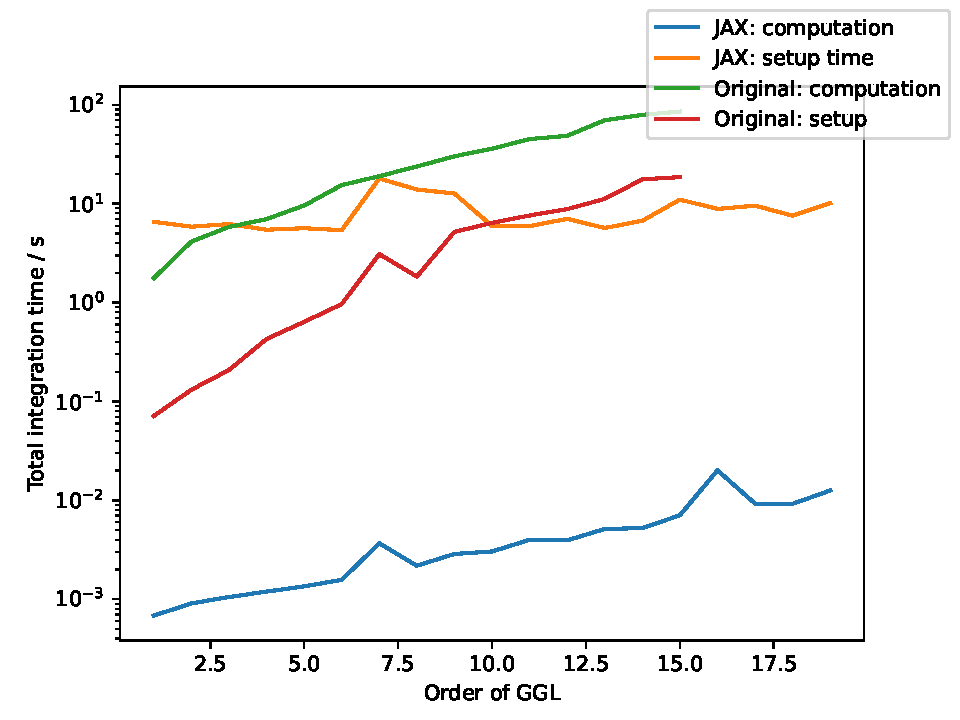
\includegraphics[width=\columnwidth]{figures/dho_r_runtime.pdf}
  \caption{A comparison of running a damped harmonic oscillator system for various values of $r$, the order of the GGL quadrature, with $\Niter = 500, \Delta t = 0.1$. Each result is the mean of 4 independent runs.
	For both implementations, we split the overall time into setup and computation as changing the method order requires re-discretising the Lagrangian and thus non-trivial work under both implementations.}
  \label{fig:dho-r-runtime}
\end{figure}

Next, we explored the time complexity of the system in terms of the iteration count, $N_{\text{iter}}$, and GGL quadrature order, $r$. These are important to physical applications as they determine the limits of iteration accuracy when iterating over large timescales -- with error scaling as $(\Delta t)^{2r + 2}$ and total timeframe being $N_{\text{iter}} \Delta t$.

Focusing first on the time complexity in $N_{\text{iter}}$ as shown in \fref{fig:dho-n-runtime}, we note that the computation time of the \updimpl{} is much lower than that of the \orgimpl{}, with the \updimpl{} growing as $\Or((\Niter)^a)$ where $a = 1.0140 \pm 0.0042$. 
In addition, we note that the fixed cost JIT compilation remains roughly constant until $10^7$ iterations after which it begins to grow linearly.

This pattern is seen also in \fref{fig:dho-r-runtime} when investigating the time complexity in the order of the method. Again the JIT time remains roughly constant across the domain tested, and though it starts initially higher than the \orgimpl{}'s setup costs, the \orgimpl{}'s computation time quickly swamps this fixed cost.
Similar to the behaviour in $\Niter$, the computation time for the \updimpl{} is also linear $r$, remaining insignificant in the overall runtime. This is in comparison with the \orgimpl{} where the setup time grows as $\Or(r^n)$ with $n = {2.31 \pm 0.15}$ and the computation time as $\Or(r^m)$ with $m={1.490 \pm 0.070}$.

It should be noted that while increasing the order of the method will increase the precision, at higher orders we start encountering limitations with the fixed precision \texttt{float64} type used for calculation in the \updimpl{} compared to the arbitrary precision numerics employed in the \orgimpl{}.
Still, however, this represents an overall improvement in accuracy in physically meaningful simulations as the required precision could be more readily attained by decreasing $\Delta t$ rather than increasing $r$, avoiding the large increase in runtime observed in the \orgimpl{}, or the degradation of precision at high $r$ in the \updimpl{}. This is discussed further in \sref{sec:results-si}
